% Needed packages
\documentclass[a4paper, 10pt, english, onecolumn]{article}
\usepackage[english]{babel}
\usepackage[cm]{fullpage}
\usepackage{cite}
\usepackage{anysize}
\usepackage{setspace}
%\usepackage[compact]{titlesec}
\usepackage{graphicx}
\usepackage{stfloats}
\usepackage{listings}
\usepackage{hyperref}

\usepackage{amssymb,amsmath}
\usepackage{algorithmicx}
%\usepackage{algorithmic}
\usepackage{algorithm}
\usepackage[noend]{algpseudocode}

% for coloring individual cells in a table
\usepackage[table]{xcolor}
%\usepackage{pgfgantt}

%\newcommand{\keywords}[1]{\par\noindent 
%{\bf Keywords\/}. #1}

% Margins & Headers
\marginsize{2.5cm}{2.5cm}{3.0cm}{2.0cm}
\columnsep 0.4in
\footskip 0.4in 
\usepackage{changepage}

% E-mail formatting
\usepackage{color,hyperref}
    \catcode`\_=11\relax
    \newcommand\email[1]{\_email #1\q_nil}
    \def\_email#1@#2\q_nil{
      \href{mailto:#1@#2}{{\emailfont #1\emailampersat #2}}
    }
    \newcommand\emailfont{\sffamily}
    \newcommand\emailampersat{{\color{red}\small@}}
    \catcode`\_=8\relax 
	
% List modifications
\newenvironment{packed_item}{
\begin{itemize}
  \setlength{\itemsep}{1pt}
  \setlength{\parskip}{0pt}
  \setlength{\parsep}{0pt}
}{\end{itemize}}

\newenvironment{packed_enum}{
\begin{enumerate}
  \setlength{\itemsep}{1pt}
  \setlength{\parskip}{0pt}
  \setlength{\parsep}{0pt}
}{\end{enumerate}}

% ### Mathematics ###
\newcommand{\bpm}{\begin{pmatrix}}
\newcommand{\epm}{\end{pmatrix}}

\newcommand{\bbm}{\begin{bmatrix}}
\newcommand{\ebm}{\end{bmatrix}}

\newcommand{\bsm}{\bigl( \begin{smallmatrix}}
\newcommand{\esm}{ \end{smallmatrix} \bigl)} 

\newcommand{\mbf}{\mathbf}

% ### Matrices and Vectors ###
\newcommand{\mtx}[1]{\ensuremath{\boldsymbol{#1}}}
\newcommand*\Let[2]{\State #1 $\gets$ #2}

% ### Sets ###
\newcommand{\set}[1]{\ensuremath{\mathcal{#1}}}

% ### Other ###

\newcommand{\transpose}{^{T}}
\newcommand{\inv}{^{-1}}
\newcommand{\pseudoinv}{^{+}}

% ### Hyphenation ###
\hyphenation{a-na-ly-sis}

% ### dots at the end of arrows and lines ###

\def \orightarrow {\circ\hspace{-0.42em}\rightarrow}
\def \oleftarrow {\leftarrow\hspace{-0.42em}\circ}
\def \orightline {\circ\hspace{-0.16em}-}
\def \oleftline {-\hspace{-0.16em}\circ}
\def \oline {\circ\hspace{-0.38em}-\hspace{-0.2em}\circ}
\def \srightarrow {\text{\textasteriskcentered}\hspace{-0.62em}\rightarrow}
\def \sleftarrow {\leftarrow\hspace{-0.62em}\text{\textasteriskcentered}}
\def \srightline {\text{\textasteriskcentered}\hspace{-0.16em}-}
\def \sleftline {-\hspace{-0.40em}\text{\textasteriskcentered}}
\def \sline {\text{\textasteriskcentered}\hspace{-0.38em}-\hspace{-0.4em}\text{\textasteriskcentered}}
\def \soline {\text{\textasteriskcentered}\hspace{-0.16em}-\hspace{-0.4em}\circ}
\def \osline {\circ\hspace{-0.38em}-\hspace{-0.16em}\text{\textasteriskcentered}}

% ############## End Macros ##############

% ### Section Formatting ###
\usepackage[compact]{titlesec}
\titlespacing*{\section}{4pt}{*0}{4pt}

% ### Paragraph Formatting ###
\makeatletter
\renewcommand{\paragraph}{%
  \@startsection{paragraph}{4}%
  {\z@}{0.5ex \@plus 1ex \@minus .2ex}{-1em}%
  {\normalfont\normalsize\bfseries}%
}
\makeatother

% Title
\title{\fontfamily{phv}\selectfont{Causal Discovery methods for Effective Connectivity in Human Brains}}
\author{
  \textbf{R. Janssen} - \href{mailto:ramon.janssen@student.ru.nl}{ramon.janssen@student.ru.nl} \\
  \textbf{T. de Ruijter} - \href{mailto:t.deruijter@student.ru.nl}{t.deruijter@student.ru.nl}\\
%  \textbf{T. Claassen} - \href{mailto:tomc@cs.ru.nl}{tomc@cs.ru.nl}\\
%  \textbf{M. Hinne} - \href{mailto:mhinne@cs.ru.nl}{mhinne@cs.ru.nl}
}

\date{\fontfamily{ptm}\selectfont{\small{\bfseries{\today - Radboud
Universiteit Nijmegen}}}\\[0.5cm]\rule{\linewidth}{0.3mm}}

\begin{document}

\maketitle

\setlength{\parindent}{0.0cm}
\setlength{\parskip}{3mm plus2mm minus1.5mm}

\begin{abstract}
% TODO: first state what you try to do, then how you did it, then what it brought you
%In this work we applied PC algorithm on resting-state data of healthy human subjects.
%Additionally we propose a variant of PC algorithm that poses weaker assumptions on the model, better fitting the underlying model.
%We find that detecting structure homological areas in the brain works better with PC algorithm than most conventional diffusion weighted imaging techniques.
%In the area of directionality and causality, more research is needed.
\end{abstract}

\section{Introduction}
% Petty introductory talk
The brain and particularly the human brain have been studied for hundreds of years.
Today, the secrets of our brains still belong to the most sought-after.
The techniques for studying it however have changed.
We have come a long way since the time of Phrenology, the pseudoscience based attempting to derive cognitive ability and personality from measurements of the skull or, post-mortem, the brain.
Advanced measurement methods exist that allow scientists to peek inside brains that give a coarse but broad overview without opening a single skull.

% Motivation for brain connectomics
The question how our brains are wired - brain connectomics - drives one of the leading fields of research in neuroscience.
Our brains are in essence networks which can be analysed similarly to very large graphs.
Neuro-degenerative diseases such as Alzheimer's disease, Parkinson's disease, dementia, Amyotrophic lateral sclerosis (ALS) have all been shown to severely alter brain connectivity \cite{Bullmore2009}.
An application of connectivity analysis would be to provide markers to identify the disease and its severity, as well as another means of studying these diseases.

% Causal discovery and brain networks
The field of brain connectivity finds its roots in the early 1990s \cite{friston1993functional, friston1994}, though because of more recent developments in the field of Artificial Intelligence and Machine Learning it is possible to do more thorough analysis \cite{vandenheuvel2010}.
Research regarding effective connectivity - causal relations in brain networks - is relatively new and its application still faces many challenges that require further research \cite{ramsey2010}.
Similarly to how graph theory has been applied in functional and anatomical brain networks, it seems natural to apply methods from causal discovery to deduce effective brain networks.

% TODO: Elaborate on the problems that exist within effective connectivity.
% From there on, go towards the problem statement and the unique contributions of this work.

\subsection{Problem statement}
% TODO: Tom: I am not a priori sure there are causal patterns in the human brain: what you try to do is see whether applying causal methods can help to bring new insights .. and perhaps to see if you can find evidence for the existence of such patterns.
This work seeks to utilise the strengths of current state-of-the-art causal discovery methods by applying them to resting state brain fMRI data in order to find new applicable methods for determining causal patterns in the human brain.

% BOLD Problem
The work by \cite{ramsey2010} addresses several problems causal analysis in fMRI analysis suffers from.
Methods in causal discovery have high computational costs, making it nearly impossible to calculate networks with more than hundreds of nodes.
Another important fact is that fMRI Analysis indirectly measures brain activity, through blood oxygenation.
The measured response is correlated to true activity levels at some point in the last few seconds.
Here lies another, perhaps the most important problem for causal discovery in brains.
The temporal lag between brain activity and the measured response - also called the haemodynamic response -
is not constant within a single subject.
This means that activity in area $A$ causing activity in area $B$ might be measured the other way around.

% Latent variable problems
As the complexity of the brain exceeds contemporary measurement techniques, models should compensate for this.
Brain models that do not account for possible latent - unmeasured - sources within the brain or other shortcomings of fMRI may suffer from noise, fail to capture underlying patterns or draw erroneous conclusions.
Solutions to this particular problem have been proposed that do account for latent sources \cite{ramsey2010, waldorp2011}.

% Multi subject problems
Another problem is the strong diversity between subjects.
Every brain is inherently different, making it non-trivial to combine subject data or even draw conclusions across subjects.
Even within a single brain it changes how different areas react over time.

% Other methods
Several methods for finding effective connectivity already exist \cite{mclntosh1994, harrison2003, friston2003, roebroeck2005}.
However, using more generally applicable causal discovery methods has not been elaborated on much.
Also, none of these provide a measure of uncertainty.
It is a fact that there are errors in any graph produced.
This is inherent to the methods and the coarseness of the measurements.
As there is no standard baseline to compare results with, a measure of uncertainty would be highly preferable.
A framework for such a probabilistic approach is introduced in \cite{claassen2012}.
% TODO: Illustrate the challenges ahead based on these current methods; what problems do they suffer from? (HRF)

% Problem statement
% TODO: Specify problem statement. Right now it is too vague and our contribution through research is very much unclear.
To our knowledge, there are not yet reliable analytical methods for causal discovery linking to true anatomical connections on a whole brain level.
Furthermore there are few methods that overcome the fluctuations in Haemodynamic Response present in any brain when performing connectivity analysis. % TODO: Check this claim.
We would like to know whether applying a standard approach such as the PC-algorithm \cite{spirtes2000}, named after its authors \textbf{P}eter Spirtes and \textbf{C}lark Glymour, can solve some of the difficulties effective connectivity suffers from.

% Structure of the rest of proposal
In the remainder of this work we discuss necessary knowledge on connectivity and causal inference.
We then discuss our strategy and present and reflect on results.

\section{Brain Connectivity}
The brain is connected in a way too complicated for contemporary measurement techniques to discover.
That is why several kinds of connectivity are considered.

\subsection{Functional connectivity}
Functional connectivity describes the statistical dependence of neuronal activity between different brain regions \cite{friston1993functional}.
This gives an insight in the organisation of the brain.
Functional connectivity is strongly time-dependent, as activity changes rapidly providing and fMRI has a low temporal resolution.
This means measured dependencies can be the result of statistical noise.
Functional connectivity can be deduced by fMRI measurements of brains performing a certain cognitive task, or in so called resting-state.
Resting-state indicates that subjects are instructed to relax without thinking of anything in particular to stimulate spontaneous brain activity.
Neural activity does not stop when not doing anything in particular.
Spontaneous behaviour induced during resting-state provide typical whole image behaviour, while performing cognitive tasks restricts activity to related areas.
Measuring resting-state thus provides an advantage when analysing brain connectivity on a global, whole brain level.
Resting-state measurements do have the disadvantage that it is difficult to check whether a subject truly is in a resting-state; it is often quite difficult not to think of anything in particular.
In practice, resting state analysis appears to work quite well \cite{Lowe2000, doria2010, Bullmore2009}.

\subsubsection{Structural connectivity}
Structural connectivity is defined as the mapping of anatomical - neural - paths in the brain between different brain regions \cite{friston1994}.
This is strongly related with functional connectivity: regions can only be functionally connected if there is a structural relation between them \cite{cabral2012}.
This intuitive relation can be demonstrated empirically \cite{vandenheuvel2009}.
Structural connectivity is less time dependent as it involves mappings of anatomical connections opposing temporal activity patterns.
For all practical purposes it is time-independent - it changes over years, and still marginally during adulthood.

Hinne et al. \cite{hinne2013} proposed a Bayesian method for estimating structural networks based on Diffusion Weighted MRI (DWI) and probabilistic tractography.
The existence of white-matter tracts does not become immediately clear from imagery alone.
Other methods rely on thresholds to estimate existence of said tracts.
The proposed method results in a measure of uncertainty about where a hypothesised connection will terminate and so provides a clearly interpretable network structure as result.

\subsubsection{Effective connectivity}
In contrast to functional and structural connectivity, effective connectivity takes into account the cause and effect of relations.
It has been described as ``the influence one neural system exerts over another'' \cite{friston1994}.
Effective connectivity indicates which brain regions stimulate other regions.
Functional time series data needs to be analysed to infer effective connectivity as cause and effect can be deduced from which event precedes which.
Granger causality is a method relying on this principle.
In brain data, this principle might not necessarily hold due to the fluctuations in Haemodynamic Response.
Nevertheless, in theory it is possible to infer effective connectivity from structural connectivity and functional data \cite{mclntosh1994, harrison2003, friston2003, roebroeck2005}.

Research has been done on inferring effective connectivity directly with several methods.
The most renowned methods are the aforementioned Granger causality \cite{roebroeck2005}, Structural Equation Modelling \cite{mclntosh1994}, Multivariate Autoregressive Modeling \cite{harrison2003} and Dynamic Causal Modelling \cite{friston2003}.
These are all methods dedicated to this problem.
These methods also suffer from similar problems of which perhaps the most important are scaling behaviour and failure to cope with fluctuating Haemodynamic Responses.
Most of these methods can only handle tens of nodes in reasonable time, which becomes problematic in realistic situations with up to tens of thousands of nodes, ideally.

\subsection{Causal Discovery}
An approach for finding effective connectivity may be found in the domain of causal discovery.
A causal discovery method uses data about events to determine which of these events are correlated, and additionally, it attempts to determine which events cause which.
% TODO: you say the definition of a causal relation is 'non-trivial' and that you will cover the 'relevant principles', but you don't actually say what you mean by 'a causal relation' (especially in the context of brain-connectivity)
The definition of a causal relation is not trivial \cite[p.20]{spirtes2000} and the relevant principles will be covered in this section.
In our context, the causal discovery methods which have been used aim at inferring a Directed Acyclic Graph (DAG).
These can be interpreted from a probabilistic and a causal perspective.
%In our case, we consider graphs that also include non-directed edges, a so called Partial DAG (PDAG).

Under the causal interpretation for a DAG $G$ a causal relation is denoted with directed edges; $X \rightarrow Y$ implies that $X$ is a direct cause of $Y$.
It is also said that $X$ is the parent of $Y$, and $Y$ is the child of $X$. 
When there is a directed path $X \rightarrow Z_1 \rightarrow Z_2 \dots \rightarrow Y$, $X$ is said to be an ancestor of $Y$ and $Y$ is a descendant of $X$.
An ancestor is an (possibly indirect) cause of its descendant.

Under the probabilistic interpretation a DAG $G$, also called a Bayesian network, represents a joint probability distribution over a set of variables $V$.
Conditional dependencies are shown by arrows between vertices.
Proportionality is shown by an undirected edge between vertices.
A provable property of these networks is the \textit{Markov Property}: every variable in $G$ is independent of its non-descendants conditioned on its parents.
This property enables us to link the field of Bayesian networks, for which useful mathematical properties exist, to the causal interpretation.

% TODO: relation CMC <-> unobserved common causes <-> 'causally insufficient models': I probably know what you try to say here, but that is not what it says right now
\paragraph{Causal Markov Condition}
A set of variables represented by a causal DAG $G$ is probabilistically independent of its non-descendants (non-effects), conditioned on its parents (direct causes).

This means that there is some underlying causal process that can be represented as a DAG $G$, which is not necessarily observed.
The Causal Markov Condition also has a converse principle we also use to reason with causality.
% TODO: Tom: what do you mean with the below?
It also means that in this process there cannot be common causes of variables that are left out.

\paragraph{Causal Faithfulness Condition}
A set of variables represented by a causal DAG $G$ does not have any conditional independencies unless entailed by the Causal Markov Condition.

This second condition means the graph correctly portrays the underlying probability distribution.
It enables us to reason about causality through reasoning with the graph through the notion of directional separation.

\paragraph{d-separation}
Two nodes $X$ and $Y$ are d-separated given nodes $S$ (with $X, Y \notin S$) if there is no path between $X,Y$ or a path from $X$ to $Y$ through $S$ for which at least one of the following holds:
\begin{itemize}
\item The path contains a structure $a \rightarrow b \rightarrow c$ such that $b$ is in $S$.
\item The path contains a structure $a \leftarrow b \rightarrow c$ such that $b$ is in $S$.
\item The path contains a structure $a \rightarrow b \leftarrow c$ (in which $b$ is called a collider) such that $b$ and its descendants are \textbf{not} in $S$.
\end{itemize}
If $X$ and $Y$ are d-separated, $S$ is called a separating set of $X$ and $Y$.
Every two independent variables have a separating set; if they are unconditionally independent, this is the empty set.

As mentioned, assuming Causal Markov Conditionionality means the underlying process cannot contain unobserved common causes.
However, we may additionally assume that observed variables are a subset of those in the underlying process, so we may have common causes.
Models having this property are called \textit{Causal Insufficient}.

Call a triple of variables $\left < X,Y,Z \right >$ an \textit{unshielded triple} if $X$ and $Z$ are adjacent to Y, but not to each other.

\paragraph{V-structure}
An unshielded triple can be oriented $X \leftarrow Y \rightarrow Z$ if and only all sets that d-separate $X$ from $Z$ do not contain $Y$.
This construction is named \textit{V-structure}.

It is very unlikely that all events which are relevant for the causal graph are measured on a neuronal level; 
even with high temporal and spatial resolutions, the entire physiology of the brain is too complex to capture.
Modelling with causal insufficiency would seem more accurate.
% TODO: Tom: v-structures X -> L <- Z in which L is latent do not lead to X <-> Y.
% Us: then what does it lead to??

In the underlying process, there exist V-structures $\left <X,L,Z \right>$ in which $L$ is latent.
When sampling from the observed distribution, we would find a relation $X \leftrightarrow Z$.
Since we assumed Causal Markov Conditionality, no feedback loops exist and all bi-directional arrows found must indicate existence of a latent confounder.

\subsection{PC Algorithm}
% Introduction to PC
The PC algorithm is a so-called constraint based method.
Starting from a fully connected undirected graph, the PC algorithm first forms structure by cutting away edges of conditionally independent variables.
In the second step, orientation rules are applied based on found separating sets and structure.
The original PC algorithm assumes causal sufficiency, excluding the existence of common confounders between nodes.
This seems unwanted when handling brain data, where one would expect a large amount of latent processes.
Also measuring methods are not yet advanced enough to measure the full detail of the brain, thus skipping over details.
In the perspective of causal inference, these missing areas can also appear as confounders.

For the following experiments we have used the causal insufficient version of PC algorithm, modified to handle latent variable as described by Spirtes, Glymour and Scheines \cite[p.165-167]{spirtes2000}.
Pseudocode for this method is shown in algorithm \ref{alg:pc_alg}.

%TODO: Add line numbers
\begin{algorithm}
\caption{PC algorithm}
\begin{spacing}{1.1}
\begin{algorithmic}
\Function{PC}{$data$}
\State connect all pairs of point in undirected graph $G$.
\Comment{Structural Part} 
\State $n \gets 0$
\While{there are connected pairs $X$, $Y$ such that $n < |\operatorname{Adjacencies}(X)\setminus\{Y\}| $}
  \ForAll{such connected pairs $X$, $Y$}
    \ForAll{subsets $S$ of $\operatorname{Adjacencies(X)}$ for which $|S| = n$}
      \If{$X$ and $Y$ are independent given $S$}
        \State remove edge $X - Y$ from G
        \State record $S$ as separating set of $X, Y$
        \State continue with the next pair $X$, $Y$
      \EndIf
    \EndFor
  \EndFor
  \State $n \gets n+1$
\EndWhile
\State $\text{PDAG} \gets G\text{, with all connections replaced by }\oline$
\Comment{Directional Part}
\ForAll{unshielded triples $\left <X, Y,Z \right> $ in $G$ }
  \If{$Y$ is not in the separating set of $X$ and $Z$}
    \State Orient $X \sline Y \sline Z$ as $X \srightarrow Y \sleftarrow Z$ in $\text{PDAG}$
  \EndIf
\EndFor
\State Apply other directionality rules from Spirtes et al. \cite[p.165-167]{spirtes2000}
\State \Return $G$ and the separating sets
\EndFunction
\end{algorithmic}
\end{spacing}
\label{alg:pc_alg}
\end{algorithm}

For finding directed edges, the PC-algorithm first finds undirected structure.
For each two non-adjacent nodes $X$ and $Y$ it also finds a minimal separating set, which is the smallest set acting as a separating set.
This is done by first assuming all nodes are connected, and then testing all pairs of nodes for independence.

The independence of $X$ and $Y$ is tested given a subset of neighbours of $X$ or $Y$ using a statistical independence test such as the Chi-square or Fisher-Z independence tests.
If such an independence is found, this subset is a separating set of $X$ and $Y$ and they are not connected.
If no such an independence is found, they are connected.
To find the minimal separating set, all subsets of neighbours are traversed in order of size; the first separating set which is found, is the minimal one.

Next, PC algorithm attempts to orient these edges.
The 'o' mark represents the entire Markov class in that edge of the graph.
Like Spirtes et al, we use a star-symbol at the end of an edge to denote that any mark may be present: an arrowhead, an "o" or an empty mark.
When an edge is oriented as an edge with a star, this denotes that this end is not changed.

The first of the directionality rules attempts to orient unshielded triples.
For a triple $\left < X,Y,Z, \right>$ to be oriented, $X$ and $Z$ should have a separating set $S$ not containing $Y$.
If so, the triple is marked a V-structure.

%After this rule which finds V-structures, the other rules are applied in no particular order.
%These rules are based on arrows that have already been found.
%\begin{itemize}
%\item If there is an edge $X \sline Y$, and if there is a directed path from $X$ to $Y$, then $X \sline Y$ can be oriented as $X \srightarrow Y$.
%\item If there are edges $X \srightarrow Y$ and $Y \sleftline Z$, if the latter is not an edge $Y \sleftarrow Z$, and if $X$ and $Z$ are not connected, orient $Y \sline Z$ as $Y \rightarrow Z$. 
%\end{itemize}

The PC-algorithm run-time is dependent on the number of dependency tests to be performed and thus it has a worst-case runtime complexity exponential in the maximal branching degree present in the graph.
For a sparse graph, PC algorithm runs fast in practice and is able to perform well on hundreds of variables.

% Stability Soundness and Non-completeness of PC
PC algorithm is not very stable, meaning it produces different output dependent on the order in which vertices are treated in the algorithm.
PC algorithm is sound, meaning that all directionality found is also correct.
However, PC algorithm is not complete, as not all types of causality can be detected.
It is shown that in practice PC algorithm works quite well, as complete algorithms, such as FCI also from Spirtes et al., require additional statistical tests which are intractable to perform for more than tens of variables.

\section{Material and Methods}
% Different adaptations of PC

% Modified PC
%\paragraph{Modified PC}
%An adaptation of PC algorithm by Spirtes et al. assumes causal insufficiency and returns a Markov equivalence class, rather than one specific instance of it.
%In literature it is this algorithm that is usually cited under the name PC Algorithm.
%This also makes PC algorithm more stable as the number of Markov equivalence classes is less than the number of times data can be permuted.
%However the order of vertex removal still plays a key role in the end result.
%This causal-insufficient version is named Modified PC.

% Conservative PC
% TODO: Put conservative PC in the previous section and leave this section for our additions and ideas.
\paragraph{Conservative PC}
The V-structure rule in PC algorithm orients unshielded triples based on a single separating set. 
Simply put, it is assumed the single found separating set is enough to show conditional independence. 
Ramsey et al. \cite{ramsey2012} introduce a weaker but still sufficient assumption for finding V-structures.
Through this weaker but still adjacency-faithful assumption, the method is more cautious than PC algorithm in drawing unambiguous conclusions on causal orientations.
That is why this method is named Conservative PC (CPC).
The resulting algorithmic changes provide better results and is able to mark incorrectly unshielded triples as unfaithful.
Sadly, CPC requires a significant amount of additional conditional independence tests, exponential in the largest branching degree of the tested structure.

% Multiple sepsets
\paragraph{Multiple Separating Sets}
The idea of CPC, to make a weaker assumption on graph faithfulness, is very potential.
% TODO: Is very potential??
Instead of doing additional tests, one could attempt to determine causal unfaithfulness with less dependency tests.
An adaptation to PC algorithm that would not increase the order of complexity is once a separating set is found, to test all other vertex subsets of the same order as well.
This finds all separating sets of the lowest order without increasing complexity.
Orienting an unshielded triple $\left<A,B,C\right>$ requires $B$ not to occur in any separating set of $(A,C)$.
By having more than one separating set, this constraint is strengthened.

% Unfaithfulness test
One could use these additional separating sets to test oriented unshielded triples for unfaithfulness, similar to CPC.
Apart from serving as a sanity check, this could serve as the basis of a repair algorithm for errors made by PC.

% Explicit test
A more explicit way to decrease faulty orientation of an unshielded triple $\left<A,B,C\right>$ is to check whether adding $B$ to a separating set of $(A,C)$ makes the pair conditionally dependent.
If so, the graph is likely to be more faithful to its modeled distribution.
% TODO: What is meant with 'likely to be more fateful'? Quantify this.

\paragraph{EMS-PC}
We have combined the above ideas into an adaptation of PC, which we refer to as Explicit Multiple Separating Set PC (EMS-PC).
Two changes have been made in this adaption with respect to modified PC as described by Spirtes et al \cite{spirtes2000}.
% TODO: line below is repetition of previous paragraph. Keep?
In the algorithm as described in section ~\ref{sec:pseudocode}, the search for a separating sets for $X$ and $Y$ stops when such a set is found; instead, EMS continues the search for more separating sets of the same order.

Also, the condition to orient $X - Y - Z$ according to the V-structure-rule has been made more strict.
As multiple separating sets have been found instead of only one, it needs to be checked whether $Y$ is in not in \emph{any} of those sets before the V-structure can be oriented.
Also, in addition to the original condition, $X$ and $Z$ are tested for d-separation given $\{Y\}$.
If they are found to be conditionally dependent, the triple is oriented as as $X \srightarrow Y \sleftarrow Z$.
As a final safe-guard, all unshielded triples are checked for unfaithfulness and marked as such if applicable using found separating sets. %TODO wat bedoel je hiermee?
% TODO: How do you mark unfaithful triples? can you spot the impact in the output?
\subsection{Pseudocode}
\label{sec:pseudocode}

The first part of the algorithm finds an undirected graph $G$ and is described in Algorithm ~\ref{code:emsstructure}.
For each pair of points which are not connected in this graph, it also finds a separating set. $\operatorname{Adjacencies} (X)$ is defined as the set of all neighbours of $X$ in the graph $G$.
This graph changes during the algorithm and so does $\operatorname{Adjacencies} (X)$.
The second part orients edges in this graph $G$ based on the separating sets, as described in Algorithm ~\ref{code:emsdirectional}.

% TODO: How is this different from the first part of algorithm 1?
% TODO: Add line numbers
\begin{algorithm}
\caption{Structure part of EMS-PC}
\begin{spacing}{1.1}
\begin{algorithmic}
\Function{Structure\_PC}{$data$}
\State connect all pairs of point in undirected graph $G$.
\State $n \gets 0$
\While{there are connected pairs $X$, $Y$ such that $n < |\operatorname{Adjacencies}(X)\setminus\{Y\}| $}
  \ForAll{such connected pairs $X$, $Y$}
    \ForAll{subsets $S$ of $\operatorname{Adjacencies(X)}$ for which $|S| = n$}
      \State test whether $X$ and $Y$ are d-separated given $S$
      \Comment{(Fisher-Z-test on $data$)}
      \If{$X$ and $Y$ are d-separated given $S$}
        \State remove the edge $X - Y$ from G
        \State record $S$ as a separating set of $X$ and $Y$
      \EndIf
    \EndFor
  \EndFor
  \State $n \gets n+1$
  
\EndWhile

\Return $G$ and the separating sets
\EndFunction
\end{algorithmic}
\end{spacing}
\label{code:emsstructure}
\end{algorithm}


% TODO: Add line numbers
\begin{algorithm}
\caption{Directional part of EMS-PC}
\begin{spacing}{1.1}
\begin{algorithmic}
\Function{Directional\_PC}{$G$, $sepsets$}
  \State $\text{PDAG} \gets G\text{, with all connections replaced by }\oline$
  \ForAll{unshielded triples $<X, Y, Z>$}
    \If{$Y$ is not in any separating set of $X$ and $Z \And X$ and $Z$ are dependent given $Y$}
      \Comment{V-structure-rule}
      \State Orient $X \sline Y \sline Z$ as $X \srightarrow Y \sleftarrow Z$ in $\text{PDAG}$
    \EndIf
  \EndFor
  \Repeat
    \ForAll{ordered, connected pairs $X$, $Y$}
      \Comment{Rule 1}
      \If{$X \osline Y$ or $X \sleftline Y$, and there is a node $Z$ such that $Z \srightarrow X$}
        \State Orient $X \sline Y$ as $X \rightarrow Y$
      \EndIf
      \Comment{Rule 2}
      \If{there is a directed path from $X$ to $Y$}
        \State Orient $X \sline Y$ as $X \srightarrow Y$
      \EndIf
    \EndFor
  \Until{no more edges are oriented}
  \State \Return PDAG
\EndFunction
\end{algorithmic}
\end{spacing}
\label{code:emsdirectional}
\end{algorithm}

%\par\vfill\break % Omdat pseudocode veel hspace nodig heeft :(
%\advance\hsize by -8cm % Retur n old margings and page height
%\advance\hoffset by 4cm % Return old margings and page height

\subsection{Experimental validation}
% Section on how we plan on demonstrating the empirical value of research.
% Full description from step 1 to final data set
% TODO: Tom: have you tested/verified whether or not your EMS-PC procedure is indeed 'more likely to be faithful'? (p6,l5)
% TODO: Max: You asked me about my opinion on the identified structure, there was hardly any formal comparison. You could easily quantify this!To keep your study reproducible, you should not base your study on an (anonymous!) 'expert' :)
% TODO: ''dit product is dermatologisch getest' - en wat kwam UIT de test? Again, you should quantify this, and do not use an anonymous expert to prove the validity of  method. If you find this difficult (or impossible), try looking at things like consistency across permutations and/or subjects.'
Our analysis consisted of two parts, corresponding to the structural and directional parts of PC algorithm.
Firstly we discerned structure by using brain resting-state time series fMRI data with structure PC.
The generated structure is the same for all variants of PC discussed and proposed, as only the first separating set is used in finding unshielded triples.
We compared the generated structure with a Bayesian inference approach on finding structural connectivity from diffusion weighted imaging.
Comparison between structures is done visually with an expert on brain anatomy.
To increase the stability of found structures within subjects, we apply stability selection for different node permutations by Meinshausen and B{\"u}hlmann \cite{meinshausen2010}.
Multi-subject comparison was done by averaging and inspecting standard deviation over subjects.
% TODO: Inspecting and concluding what?

The second part of our analysis is about discerning orientation within the found structure.
We applied the directionality rules of original PC, modified PC and EMS-PC as mentioned above.
Resulting connectivity patterns are visually compared by an expert for anatomical correctness.
To compare between methods, we compare the consistency of methods to mark a specific connection as directional over permutations.
Of specific interest here are non-symmetrical orientations.
We again applied stability selection for a sufficiently large number of permutations per subject.
% TODO: How do you determine 'sufficient' and what is this number?

\subsection{Data acquisition}
% TODO: Huh? No data acquisition? Where do you get your results from then?
No explicit data acquisition was performed, instead we performed our analysis on the same data as treated by Hinne et al. in the aforementioned Bayesian structural analysis \cite{hinne2013, hinne2013structfunc}.

% TODO: Paraphrase this, instead of quoting.
Quoting: ``six healthy volunteers were scanned for resting-state functional data and diffusion-weighted images using a Siemens Magnetom Trio 3 T system at the Donders Centre for Cognitive Neuroimaging at Radboud University in The Netherlands.
Resting-state fMRI data were acquired at 3 Tesla by using a multi-echo echo-planar imaging (ME-EPI) sequence (voxel size 3.5 mm isotropic, matrix size 64x64, TR=2000 ms, TEs=6.9, 16.2, 25, 35 and 45 ms, 39 slices, GRAPPA factor 3, 6/8 partial Fourier).
A total of 1030 volumes were obtained.
Diffusion weighted images were obtained by using the DWI protocol (voxel size 2.0 isotropic, matrix size 110x110, TR=13.00 ms, TE=101 ms, 70 slices, 256 directions at b=1500 s/mm$^2$).''

% TODO: There was a lot (!) of pre-processing conducted after the data was collected. You should emphasise this and refer the reader to the original article so look these things up, if desired.
We did not perform explicit (pre-)processing on the functional and diffusion imaging data.
Instead, we used the six resulting resting-state functional time series data and connectivity matrices from the Bayesian analysis as (pre-)processed by Hinne et al. \cite{hinne2013}.
% K is de MAP estimate uit een G-Wishart distributie. Dat wil zoveel zeggen als: een distributie over alle precisiematrices die nullen hebben op de plekken waar G een 0 heeft (Hastie, Trevor; Tibshirani, Robert; Friedman, J. (2009). The Elements of Statistical Learning, voor de ge�nteresseerden). 

\section{Results}
% TODO: I'm missing a clear answer to the question "did we manage to do what we set out to do"?
At first, we have applied modified PC on the structural connectivity data of six subjects.
To achieve stability, we have run the algorithm multiple times, in which the data was permuted randomly in each iteration.
The avarage of all iterations was used as a measure of certainty, i.e. how consistent the algorithm is for each point of data.

The results from the agorithms are presented in the form of matrices.
A connection from region $n$ to region $m$ is represented by point $(n,m)$ or $n,m$ in the matrix.
For structural data, this matrix is therefore symmetrical.
In the directional data, point $(n,m)$ denotes a directed edge from $n$ to $m$.
In such a matrix, indices 1-45 represent the brain regions of the left hemisphere, regions 45-90 represent the right hemisphere, and regions 91-116 represent regions in the cerebellum.
Modified PC and EMS-PC do not differ in finding the structure.

%  uit een merge-conflict die ontstaan is bij de haastige inleverpoging van de vorige deadline
%The results are presented in figure ~\ref{fig:struct_avg} as the avarage over all six subjects, with 300 iterations per subject.
%The results of Hinne et al. are shown in ~\ref{fig:struct_max} for comparison.

%\begin{figure}[h!]
%  \centering
%  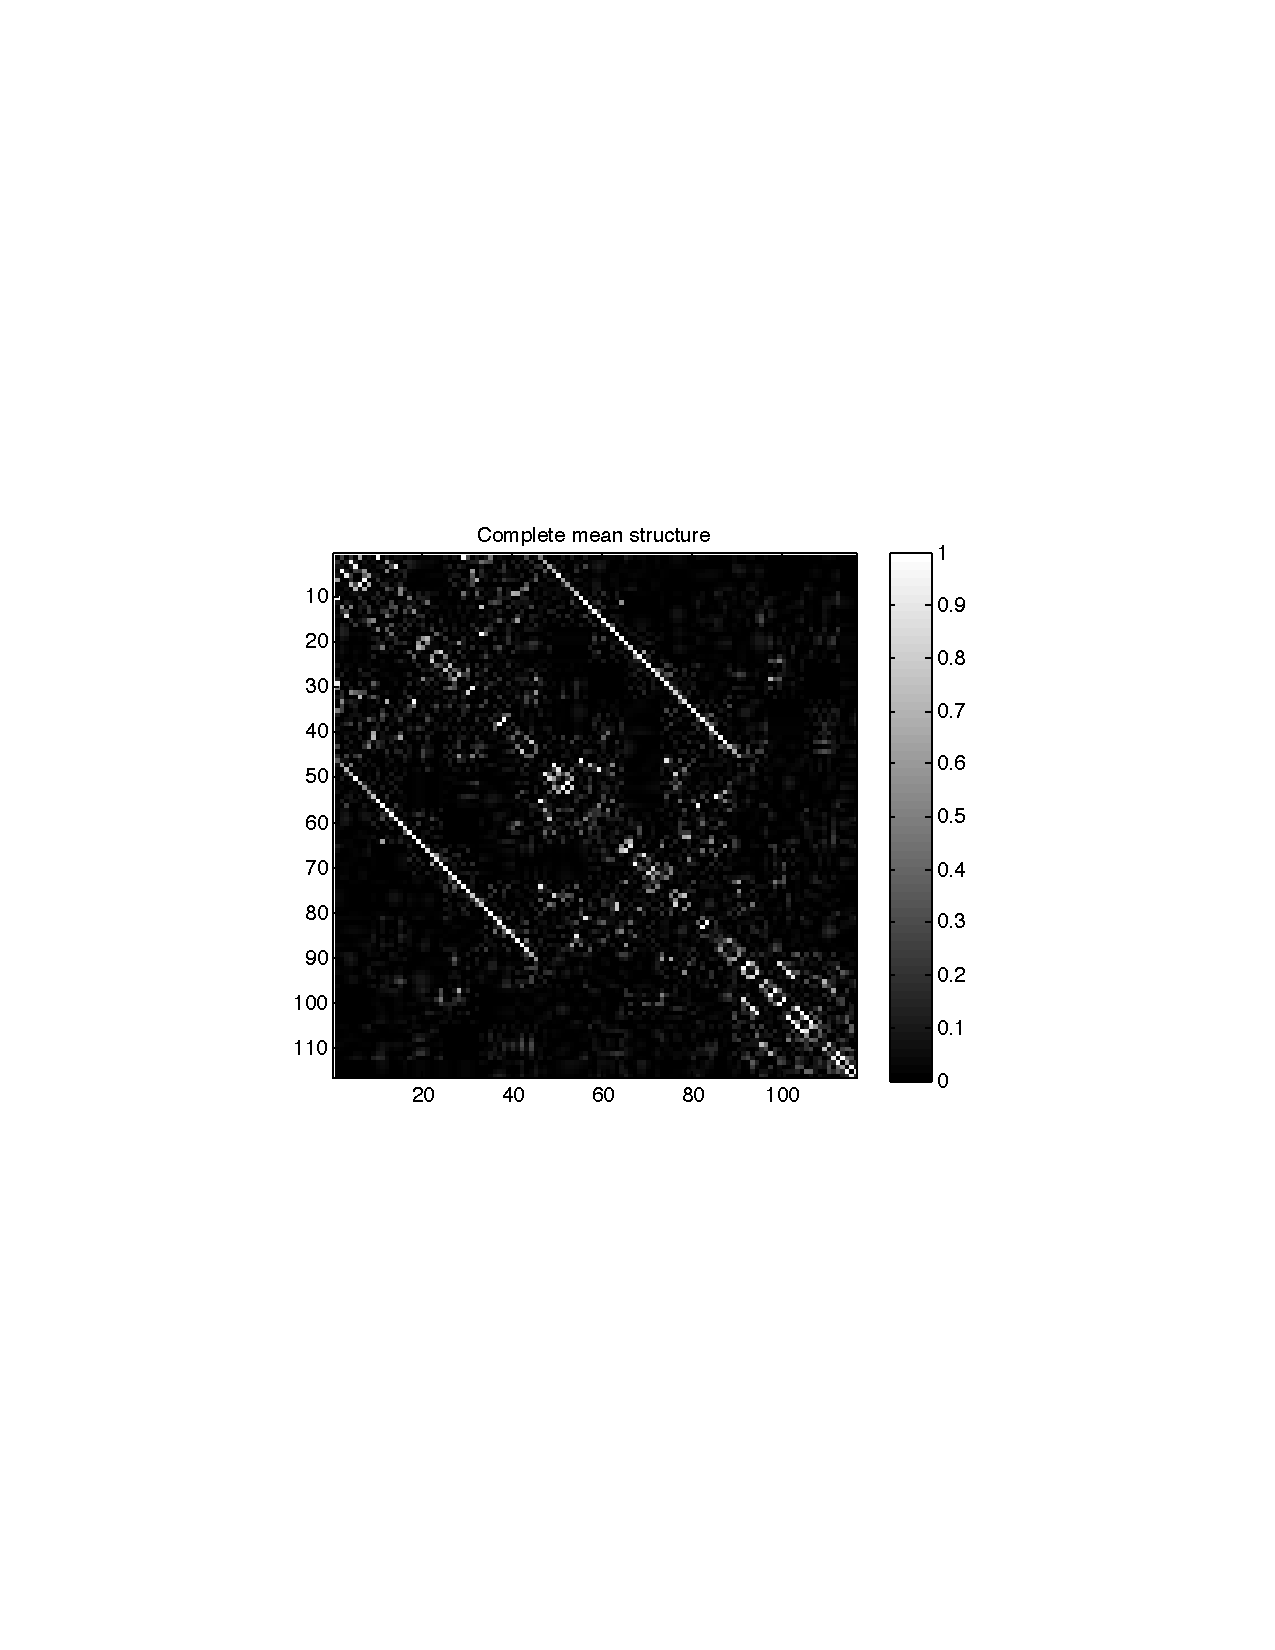
\includegraphics{images/struct_full_mean_gray}
%  \caption{The avarage structure of all subjects, found with the PC-algorithm}
%  \label{fig:struct_avg}

The results are presented in figure ~\ref{fig:struct_avg} as the average over all six subjects, with 300 iterations per subject. Additionally, separate parts of the two hemispheres, the inter-hemisphere, and the cerebellum are presented in Figures \ref{fig:struct_left}, \ref{fig:struct_right}, \ref{fig:struct_inter_hemisphere}, \ref{fig:struct_cerebellum}, \ref{fig:struct_apart}
The results of Hinne et al. are shown as well for comparison.

% TODO: Add in caption what the reader is supposed to be looking at.
\begin{figure}[h!]
  \centering
  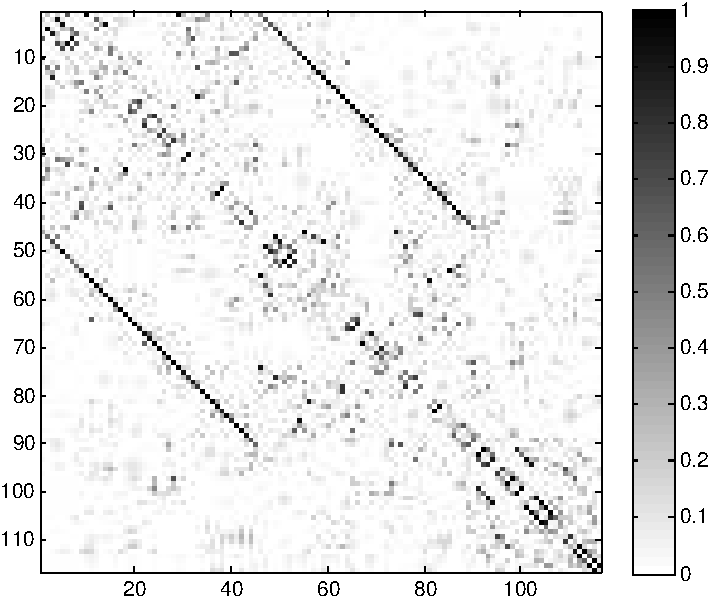
\includegraphics[width=0.5\textwidth]{images/struct_full}
  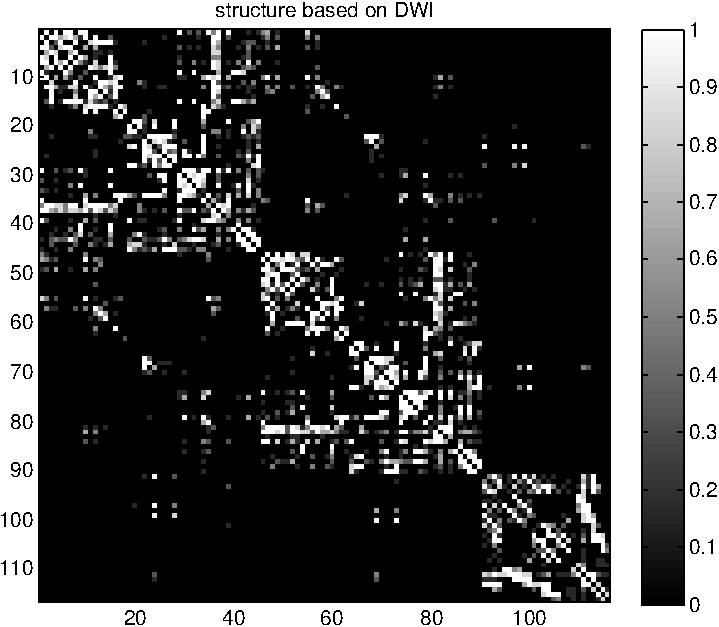
\includegraphics[width=0.5\textwidth]{images/structure_max}
  \caption{The avarage structure of all subjects. The structure on the left is found with the PC-algorithm, and the structure on the right is found with DWI-measurements by Hinne et al.}
\label{fig:struct_avg}
\end{figure}
In this matrix, higher values represent strong certainties of the presence of a connection.

end{figure}

%<<<<<<< HEAD
%\begin{figure}[h!]
%  \centering
%  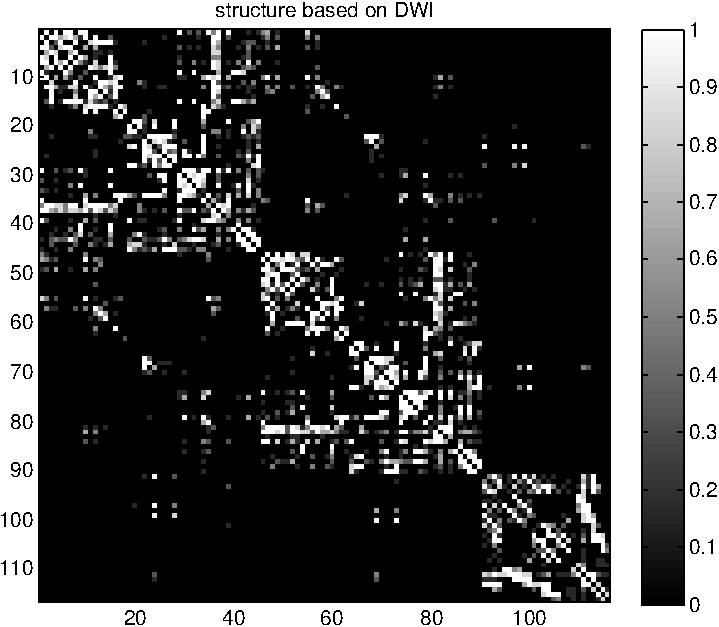
\includegraphics{images/structure_max}
%  \caption{The avarage structure of all subjects, according to the DWI-measurements of Hinne et al.}
%  \label{fig:struct_max}
%\end{figure}

One notable difference between the results found in Hinne et al. is the strong connections between homological areas, visible as two diagonal lines.
This is a known shortcoming of diffusion weighted imaging, as these connections are typically too long to measure correctly.
These connections most likely correspond to the corpus callosum, as each region is connected with its counterpart in the other hemisphere.
Connections within the hemispheres are less clearly visible, as well as connections within the cerebellum.

The second step of the PC-algorithm finds directions based on this structure.
In Figures ~\ref{fig:pdag_avg_mod} and ~\ref{fig:pdag_avg_ems}, the results for both modified PC and EMS-PC are presented.
The figures look very similar to the Figure ~\ref{fig:struct_full_mean}, and look strongly symmetric.
In terms of causality, this means that many latent sources are still present and causal relations between the measured brain regions themselves are not clearly visible.

%\begin{figure}[h!]
%  \centering
%  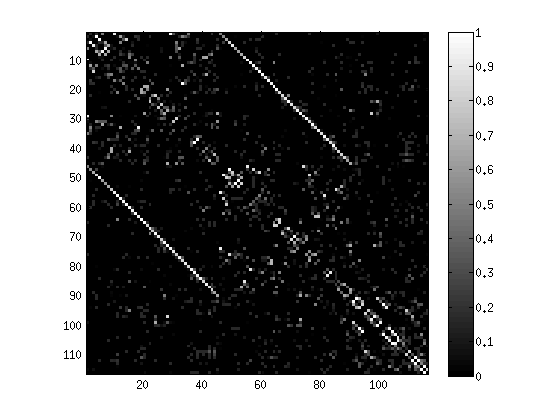
\includegraphics{images/PDAG_avg_mod}
%  \caption{The PDAG found with modified PC, in which a high value denotes a high certainty of an arrow. The avarage of all six subjects is taken.}
%  \label{fig:pdag_avg_mod}
%=======
\begin{figure}[h!]
  \centering
  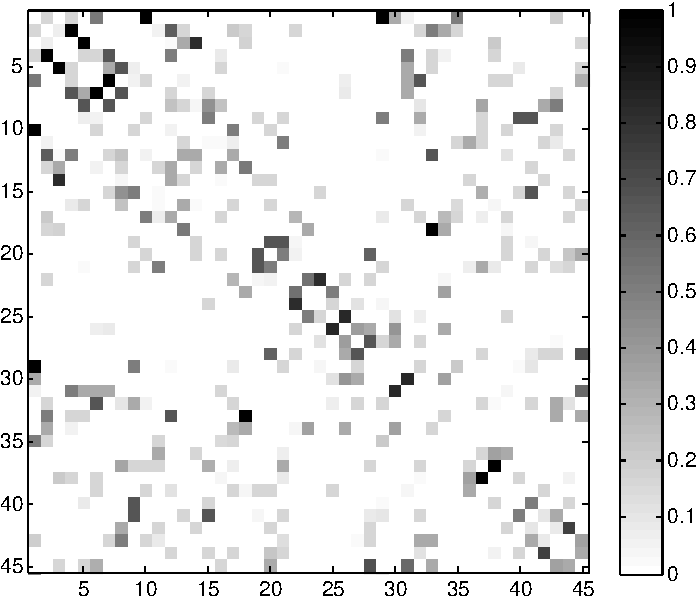
\includegraphics[width=0.25\textwidth]{images/struct_hemisphere_1_45}
  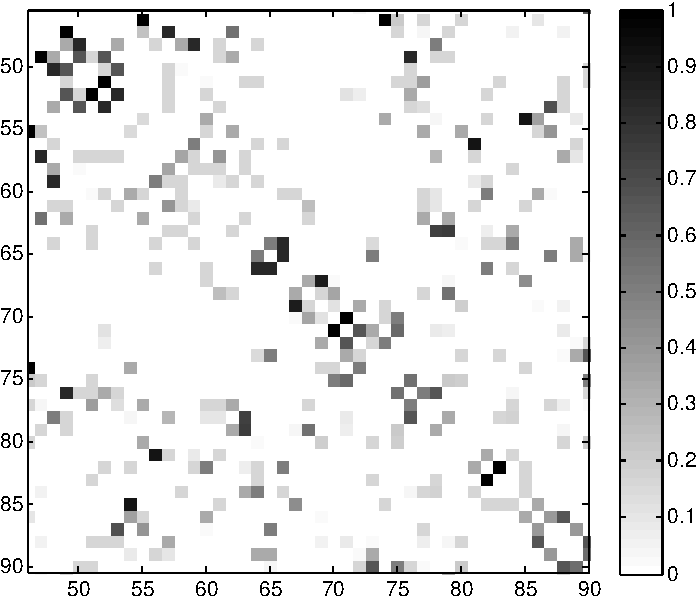
\includegraphics[width=0.25\textwidth]{images/struct_hemisphere_46_90}
  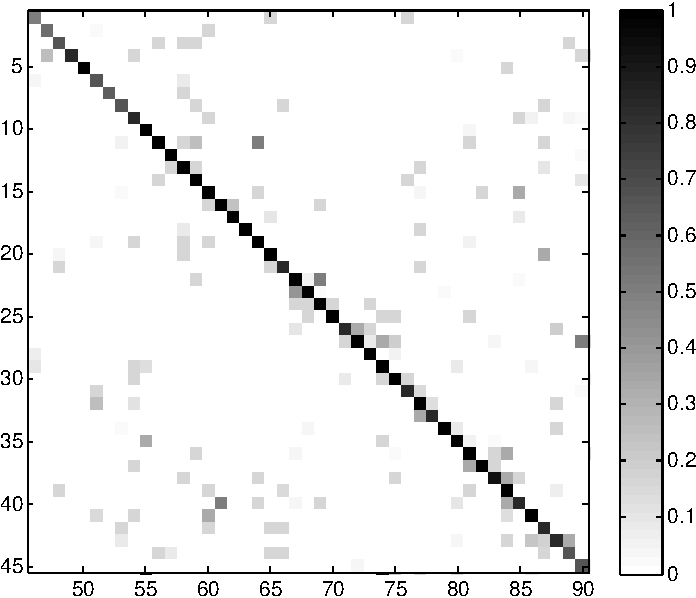
\includegraphics[width=0.25\textwidth]{images/struct_inter_hemisphere}
  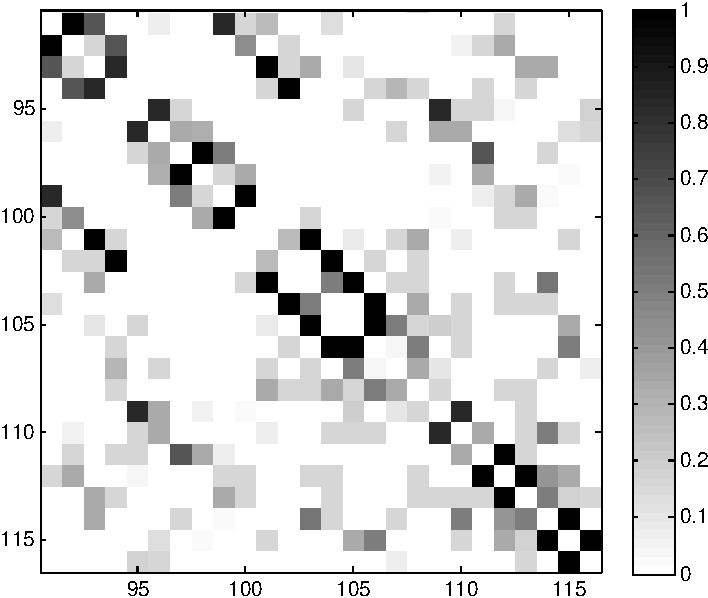
\includegraphics[width=0.25\textwidth]{images/struct_cerebellum}  
  \caption{The average structure of the left and right hemisphere, the inter-hemisphere, and the cerebellum of all subjects, as found with PC.}
  \label{fig:struct_apart}
\end{figure}

% TODO: hard to compare or see what to look for -> "does it make sense or not"?
\begin{figure}[h!]
  \centering
  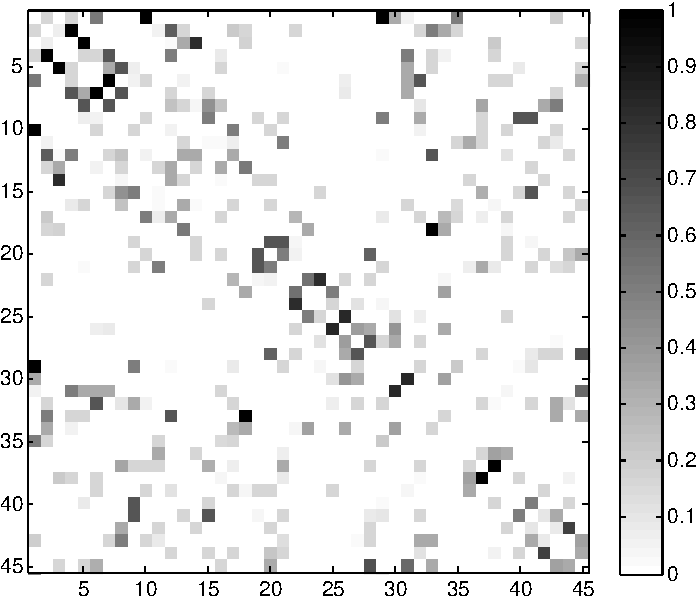
\includegraphics{images/struct_hemisphere_1_45}
  \caption{The average structure of the left hemisphere of all subjects, as found with PC.}
  \label{fig:struct_left}
\end{figure}
\begin{figure}[h!]
  \centering
  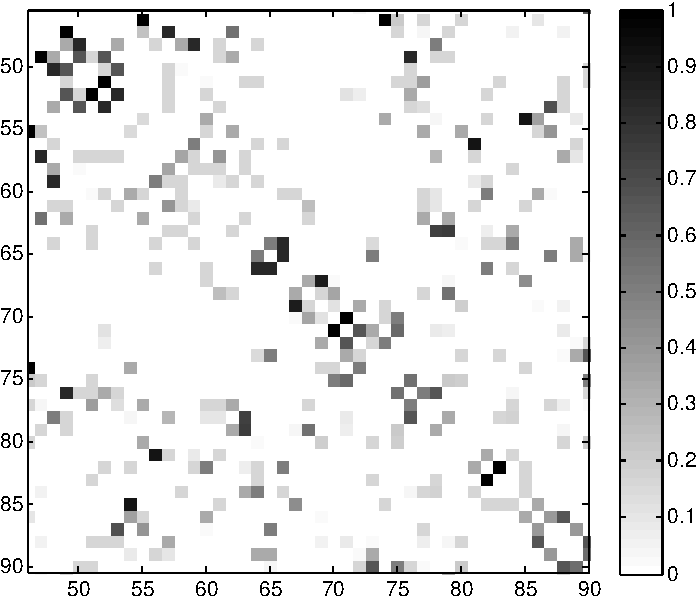
\includegraphics{images/struct_hemisphere_46_90}
  \caption{The average structure of the right hemisphere of all subjects, as found with PC.}
  \label{fig:struct_right}
\end{figure}
\begin{figure}[h!]
  \centering
  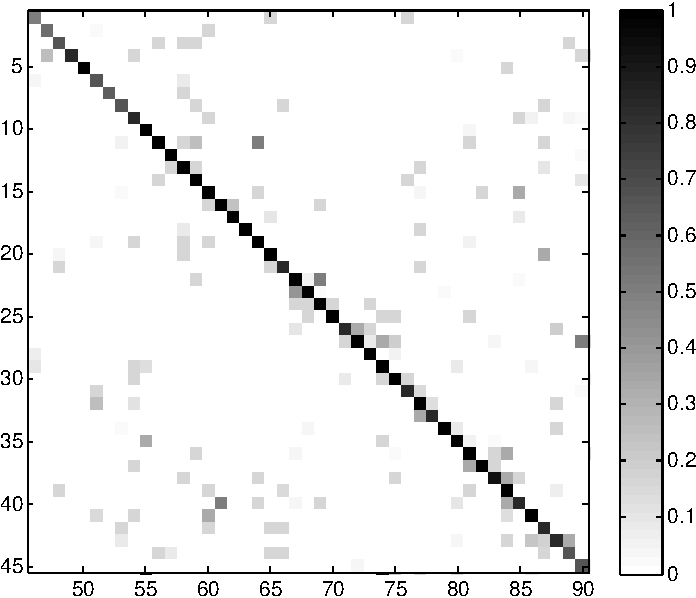
\includegraphics{images/struct_inter_hemisphere}
  \caption{The average structure between the two hemispheres of all subjects, as found with PC.}
  \label{fig:struct_inter_hemisphere}
\end{figure}
\begin{figure}[h!]
  \centering
  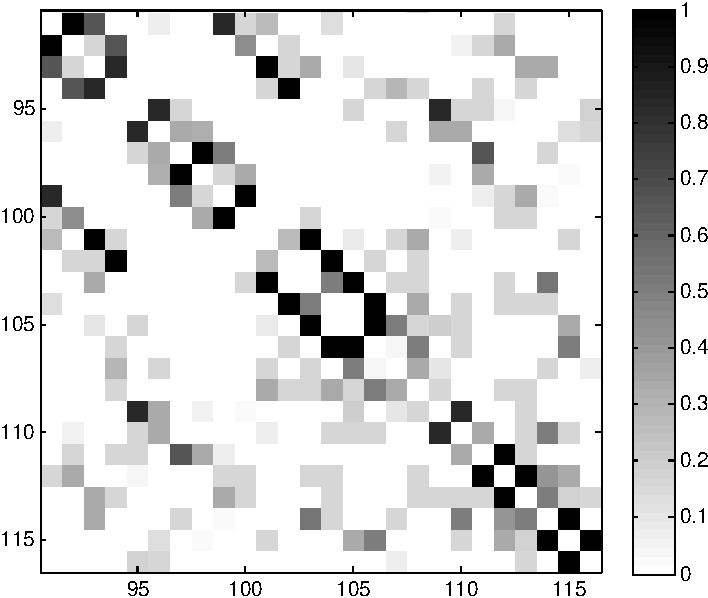
\includegraphics{images/struct_cerebellum}
  \caption{The average structure of the cerebellum of all subjects, as found with PC.}
  \label{fig:struct_cerebellum}
\end{figure}

The connections between the homologous areas are clearly visible as two diagonal lines.
These connections might run through the corpus callosum, as each region is connected with its counterpart in the other hemisphere.
However the matrix does not show concrete pathways so it is impossible to draw any definite conclusions on this based on just these figures.
Compared to the structure found by Hinne et al, connections within the hemispheres are less clearly visible, as well as connections within the cerebellum.

The second step of the PC-algorithm finds directions based on this structure.
In Figures ~\ref{fig:pdag_avg_mod} and ~\ref{fig:pdag_avg_ems}, the results for both modified PC and EMS-PC are presented.
The figures look very similar to Figure ~\ref{fig:struct_avg}, and look strongly symmetric.
In terms of causality, this means that many latent sources are still present and causal relations between the measured brain regions themselves are not clearly visible.

\begin{figure}[h!]
  \centering
  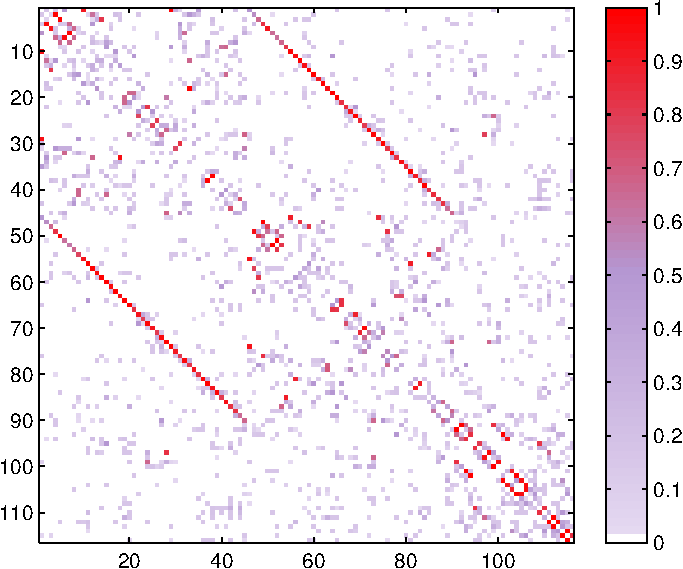
\includegraphics{images/pdag_avg_colored_mod}
  \caption{The PDAG found with modified PC, in which a high value denotes a high certainty of an arrow. The avarage of all six subjects is taken.}
  \label{fig:pdag_avg_mod}
\end{figure}

\begin{figure}[h!]
  \centering
  \includegraphics{images/PDAG_avg_colored_expl}
  \caption{The PDAG found with EMS-PC, in which a high value denotes a high certainty of an arrow. The avarage of all six subjects is taken.}
  \label{fig:pdag_avg_ems}
\end{figure}

Another representation of this data has been used to emphasise the asymmetric parts of Figures ~\ref{fig:pdag_avg_mod} and ~\ref{fig:pdag_avg_ems}.
To achieve this, the absolute difference between these matrices and their transpose has been calculated, lifting out those points for which there is an arrow in one direction, but not in the opposite direction.
These resulting antisymmetric matrices are presented in Figures ~\ref{fig:pdag_avg_antisymmetric_mod} and ~\ref{fig:pdag_avg_antisymmetric_ems}.

\begin{figure}[h!]
  \centering
  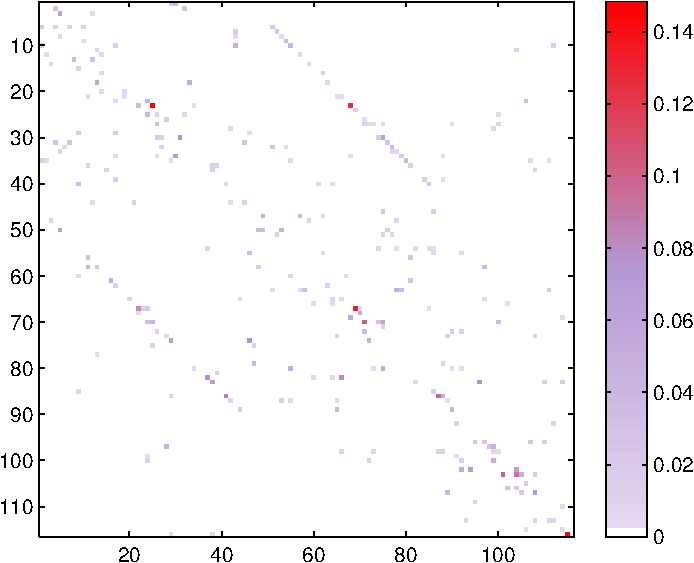
\includegraphics{images/arrowheads_avg_mod}
  \caption{The asymmetric arrowheads of the PDAG found with modified PC, in which a high value denotes a high certainty of an one-directional arrow. The average of all six subjects is taken.}
  \label{fig:pdag_avg_antisymmetric_mod}
%>>>>>>> 6d0d26f13f6a0b4326b7a5c962d4444f78f8d2ea
\end{figure}

\begin{figure}[h!]
  \centering
%<<<<<<< HEAD
%  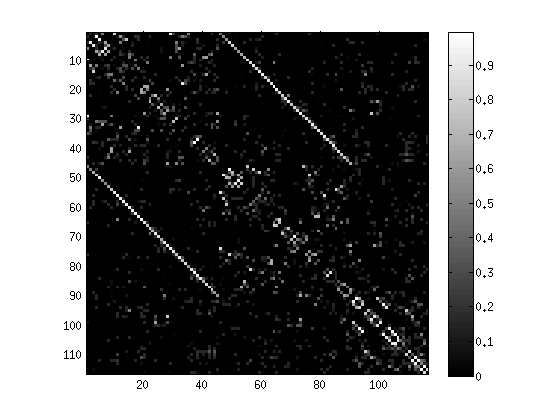
\includegraphics{images/PDAG_avg_expl}
%  \caption{The PDAG found with EMS-PC, in which a high value denotes a high certainty of an arrow. The avarage of all six subjects is taken.}
%  \label{fig:pdag_avg_ems}
%\end{figure}

%Another representation of this data has been used to emphasize the assymetric parts of Figures ~\ref{fig:pdag_avg_mod} and ~\ref{fig:pdag_avg_ems}.
%To achieve this, the absolute difference between these matrices and their transpose has been calculated, lifting out those points for which there is an arrow in one direction, but not in the opposite direction.
%These results are presented in Figures ~\ref{fig:pdag_avg_antisymmetric_mod} and ~\ref{fig:pdag_avg_antisymmetric_ems}.

%\begin{figure}[h!]
%  \centering
%  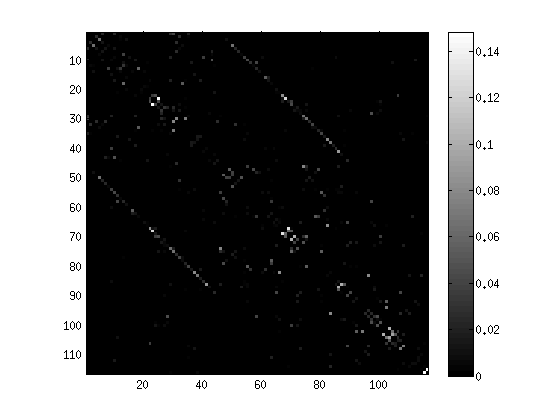
\includegraphics{images/PDAG_avg_antisymmetric_mod}
%  \caption{The assymetric parts of the PDAG found with modified PC, in which a high value denotes a high certainty of an one-directional arrow. The avarage of all six subjects is taken.}
%  \label{fig:pdag_avg_antisymmetric_mod}
%\end{figure}
%=======
  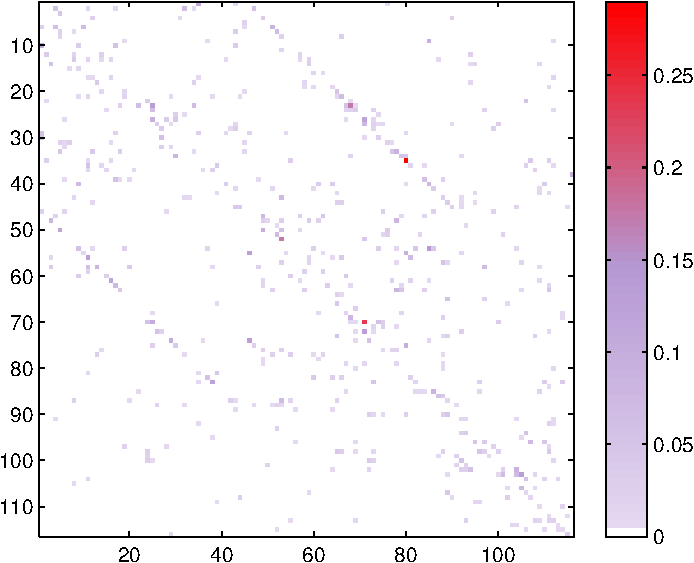
\includegraphics{images/arrowheads_avg_expl}
  \caption{The asymmetric arrowheads of the PDAG found with EMS-PC, in which a high value denotes a high certainty of an one-directional arrow. The average of all six subjects is taken.}
  \label{fig:pdag_avg_antisymmetric_ems}
\end{figure}

A notable difference between modified PC and EMS-PC is that the asymmetric arrowheads of the PDAG are about twice as high. %TODO: histogram
This means that with our data, EMS-PC finds more arrows pointing in only one direction, and it finds them more consistently.
However, none of these arrows are consistent among the six subjects.
This can also be concluded from the maximum values of these matrices of the individual subjects.
These matrices have maximum values of 0,45 - 0,9, whereas the average of these matrices has a maximum value of 0,25.
% TODO: That is not too worrying for this type of data. There is probably no consistent cognitive process clearly visible in this timescale, during rest.
Also, based on physiology we would expect causal relations within homologous areas to be roughly the same, but this is also cannot be concluded from our results.

\subsection{Execution time of the algorithm}
To apply the algorithms on our data, we have used a Xeon E5-2670, running on 2,6GHz.
To run one iteration of the PC algorithm for one subject, modified PC needed approximately one minute and EMS-PC needed approximately two minutes to find both structure and direction.
Although PC is not designed to be multithreaded, running multiple iterations lends itself for using multiple threads, as the iterations are fully independent, and only need to be averaged out afterwards.
%>>>>>>> 6d0d26f13f6a0b4326b7a5c962d4444f78f8d2ea

\begin{figure}[h!]
  \centering
  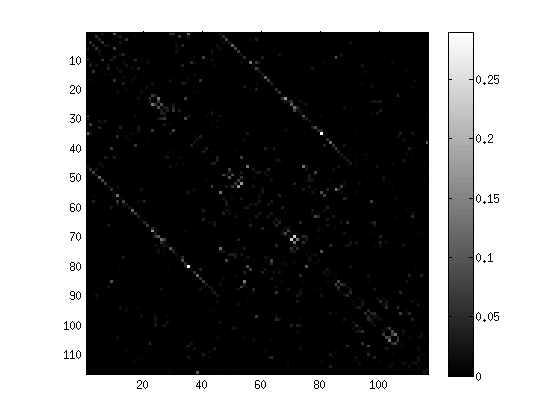
\includegraphics{images/PDAG_avg_antisymmetric_expl}
  \caption{The assymetric parts of the PDAG found with EMS-PC, in which a high value denotes a high certainty of an one-directional arrow. The avarage of all six subjects is taken.}
  \label{fig:pdag_avg_antisymmetric_ems}
\end{figure}

\section{Discussion}
The structural part of PC adds interesting information with respect to existing methods such as DWI.
Although DWI finds more structural data within homological areas, it does not find the corpus callosum, which is very clearly visible in the structure found with PC.
This is a known shortcoming of diffusion weighted imaging, as these connections are typically too long to measure correctly.
As such, causal discovery methods can contribute additional information to finding structural connectivity.

Both modified PC and EMS-PC can add directional information.
Both algorithms find many bi-directional arrows, and also some one-directional arrows.
There does not seem to be any consistency among these one-directional arrows  between different subjects, or between the two hemispheres of the same subject.
No clear conclusions can therefore be drawn yet about causality between different brain regions.

% Further research
% TODO: What do you mean with this is not necessarily noise?
This does not necessarily imply that this data is noise, as communication between brain regions might actually differ per subject.
Activity of a brain region varies strongly over time and even though the subject have attempted to be in resting state, any thought or movement may cause signals to be measured.
This leads to inconsistent directional edges, even in an algorithm which finds causal relations correctly.
Further research may be done to investigating whether any of these arrows have a physiological meaning.
This can be done by repeating these experiment with more subjects to get a better view on the significance of the directional edges.

A Bayesian network cannot contain cycles, as that would imply that a variable is it's own ancestor and thus it's own cause.
The theory used here does not incorporate a temporal component and 
Ideally, a causal discovery methods finds only directed edges, resulting in a directed acyclic graph (DAG).
%In practice, however, often not all causal relations can be inferred and undirected edges are also used in a graph.
%As such, the result of a causal discovery method is a partially directed acyclic graph (PDAG).
% TODO: What do you mean with the below sentence?
As contemporary measuring techniques are too coarse and slow to model a brain at one point in time, correctly modelling variables over multiple points in time - opposing the acyclic assumption - would provide an interesting direction of further research.

% TODO: What do you mean with 'it can also do this'? What does 'this' refer to?
It can also do this quite efficiently, as a few hundred iterations can be run in a matter of hours per subject.
We have not performed a statistical analysis on the number of iterations needed to stabilise the results.
It may be possible that a significant result can already be found with much less iterations.

% TODO: Suggereren task based analysis ipv resting state voor beter causaal beeld. 
% TODO: Maak duidelijk welke aannames gedaan worden in welke PC variant en welke aannames verzwakt zouden kunnen worden.

% TODO: Tom suggereert dat dit te veel van het goede is.
\section{Acknowledgements}
We would like to thank Max Hinne and Tom Claassen, for without them this research would not have been viable.
They have provided us with ideas, valuable discussion and the data to perform actual research.

\bibliography{references}{}
\addcontentsline{toc}{section}{References}
\bibliographystyle{plain}

\end{document}